\section{Related Work}

\subsection{Multi-task Information Extraction}

Multi-task IE is a popular research topic in recent years.
The main idea is to use a single model to perform multiple IE tasks.
IE tasks could be formulated as different graph structures.
\citet{w2ner} formulate flat, nested, and discontinuous NER tasks as a graph with next-neighboring and tail-to-head connections.
Maximal cliques also have been used to flat \& discontinuous NER tasks \cite{mac-discontinuous-ner} and trigger-available \& trigger-free event extractions \cite{ptpcg}.
DyGIE++ takes NER, RE and EE tasks as span graphs, and apply iterative propagation to enhance spans' contextual representations \cite{dygiepp}.
OneIE uses the similar graph structures with global constraint features \cite{oneie}.

\begin{figure*}[t]
    \centering
    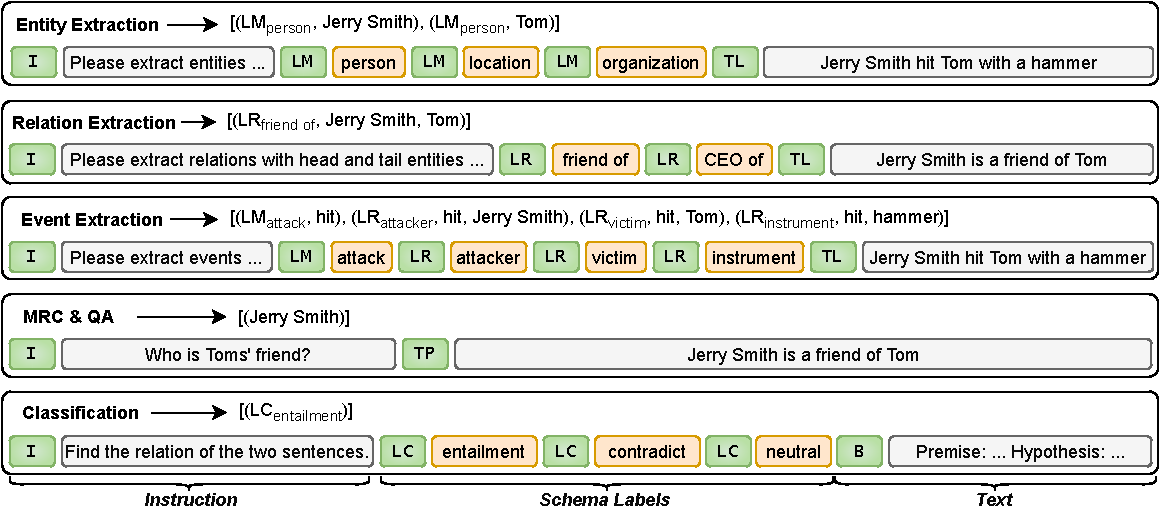
\includegraphics[width=\textwidth]{figs/inputs.pdf}
    \caption{Unified data interface.}
    \label{fig:unified-data-interface}
\end{figure*}

In addition to explicit graph-based multi-task IE systems, generative language models are also been widely used.
\citet{bart-ner} and \citet{bart-absa} add special index tokens into BART \cite{bart} vocabulary to help perform various NER and ABSA tasks and obtain explicit span positions.
TANL \cite{tanl} apply T5 \cite{t5} to generate texts with special enclosures as the predicted information.
GenIE \cite{genie} and DeepStruct \cite{deepstruct} share a similar idea to generate subject-relation-object triplets, and DeepStruct extends the model size to 10B with GLM as the backbone \cite{glm}.

\subsection{Schema-guided Information Extraction}

In schema-guided IE systems, schemas are input as an guidance signal to help the model extracting target information.
UIE \cite{uie} categorize IE tasks into span spotting and asscociating elementary tasks and devise a linearized query language.
\citet{lasuie} introduces the hyper relation extraction task to represent complex IE tasks like EE, and utilize external parsing tools to enhance the text representations.
InstructUIE \cite{instructuie} formulates schemas into instructions and uses FlanT5-11B \cite{flan-t5} to performing multi-task instruction tuning.

While the above methods use flexible generative language models, they cannot predict exact positions, which brings ambiguity when evaluating.
Besides, large generative language models are usually slow to train and inference, and requires tons of computing resources.
% USM \cite{usm} and UniEX \cite{uniex} utilize BERT-family models to extract triplets non-autoregressively.
USM \cite{usm} utilizes BERT-family models to extract triplets non-autoregressively.
USM regards IE tasks into a unified schema matching task and use a label-text matching model to extract triplets.
% UniEX inherits the idea and uses a triaffine module to predict hyper-dimensional links.
% Beyond triplets extraction, RexUIE \cite{rexuie} perform to extract n-ary tuples step-by-step.
% Although RexUIE supports n-ary extraction, it sacrifices the efficiency and requires more time when predicting results (one slot per step).
However, these methods cannot extend more information extraction tasks, such as multi-span discontinuous NER, and n-ary information extractions.
